\documentclass{standalone}
\usepackage{tikz}
\usetikzlibrary{patterns}
\usetikzlibrary{positioning}
\usetikzlibrary{patterns, positioning}
\usetikzlibrary{shapes.misc}
\usepackage[outline]{contour}
\contourlength{1.5pt} 
\usepackage[sfdefault]{ClearSans}

\begin{document}
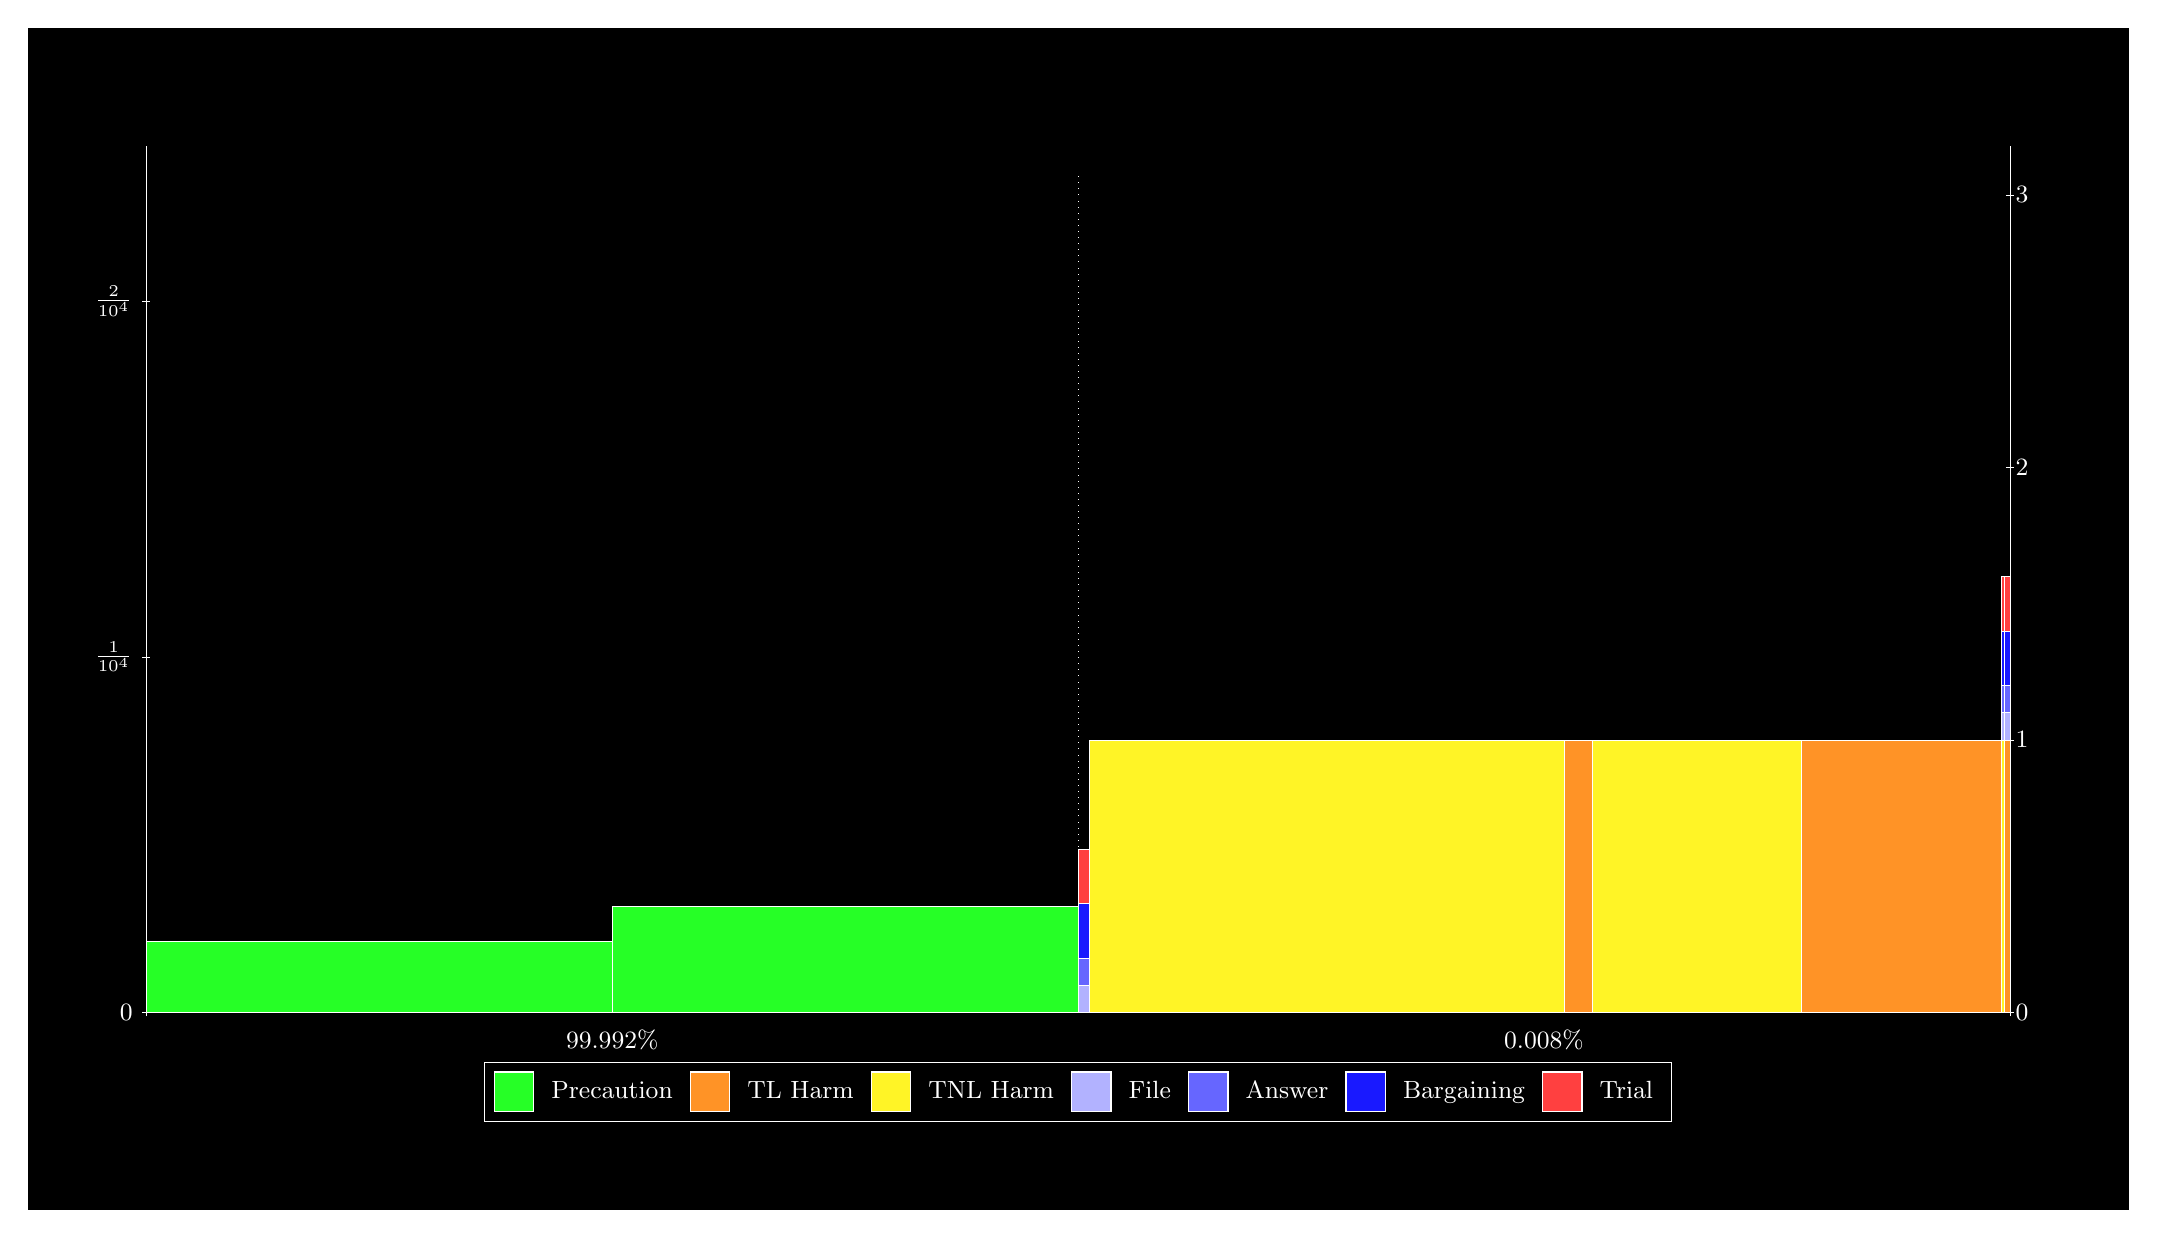
\begin{tikzpicture}
\draw[fill=black] (0,0) rectangle (26.667,15);
\draw[fill=green!85,draw=white,very thin] (1.5,2.5) rectangle (7.4166,3.4033);
\draw[fill=green!85,draw=white,very thin] (7.4166,2.5) rectangle (13.333,3.855);
\draw[fill=green!85,draw=white,very thin] (13.333,2.5) rectangle (13.481,2.5001);
\draw[fill=blue!30,draw=white,very thin] (13.333,2.5001) rectangle (13.481,2.8462);
\draw[fill=blue!60,draw=white,very thin] (13.333,2.8462) rectangle (13.481,3.1923);
\draw[fill=blue!90,draw=white,very thin] (13.333,3.1923) rectangle (13.481,3.8845);
\draw[fill=red!75,draw=white,very thin] (13.333,3.8845) rectangle (13.481,4.5767);
\draw[fill=green!85,draw=white,very thin] (13.481,2.5) rectangle (19.511,2.5001);
\draw[fill=yellow!85,draw=white,very thin] (13.481,2.5001) rectangle (19.511,5.9612);
\draw[fill=green!85,draw=white,very thin] (19.511,2.5) rectangle (19.86,2.5001);
\draw[fill=orange!85,draw=white,very thin] (19.511,2.5001) rectangle (19.86,5.9612);
\draw[fill=green!85,draw=white,very thin] (19.86,2.5) rectangle (22.513,2.5001);
\draw[fill=yellow!85,draw=white,very thin] (19.86,2.5001) rectangle (22.513,5.9612);
\draw[fill=green!85,draw=white,very thin] (22.513,2.5) rectangle (25.052,2.5001);
\draw[fill=orange!85,draw=white,very thin] (22.513,2.5001) rectangle (25.052,5.9612);
\draw[fill=green!85,draw=white,very thin] (25.052,2.5) rectangle (25.09,2.5001);
\draw[fill=yellow!85,draw=white,very thin] (25.052,2.5001) rectangle (25.09,5.9612);
\draw[fill=blue!30,draw=white,very thin] (25.052,5.9612) rectangle (25.09,6.3073);
\draw[fill=blue!60,draw=white,very thin] (25.052,6.3073) rectangle (25.09,6.6534);
\draw[fill=blue!90,draw=white,very thin] (25.052,6.6534) rectangle (25.09,7.3456);
\draw[fill=red!75,draw=white,very thin] (25.052,7.3456) rectangle (25.09,8.0378);
\draw[fill=green!85,draw=white,very thin] (25.09,2.5) rectangle (25.167,2.5001);
\draw[fill=orange!85,draw=white,very thin] (25.09,2.5001) rectangle (25.167,5.9612);
\draw[fill=blue!30,draw=white,very thin] (25.09,5.9612) rectangle (25.167,6.3073);
\draw[fill=blue!60,draw=white,very thin] (25.09,6.3073) rectangle (25.167,6.6534);
\draw[fill=blue!90,draw=white,very thin] (25.09,6.6534) rectangle (25.167,7.3456);
\draw[fill=red!75,draw=white,very thin] (25.09,7.3456) rectangle (25.167,8.0378);
\draw[white,very thin] (1.5,2.5) -- (1.5,13.5);
\draw[white,very thin] (1.45,2.5) -- (1.55,2.5);
\node[font=\small,text=white, anchor=east] at (1.45, 2.5) {0};
\draw[white,very thin] (1.45,7.0166) -- (1.55,7.0166);
\node[font=\small,text=white, anchor=east] at (1.45, 7.0166) {$\frac{1}{10^{4}}$};
\draw[white,very thin] (1.45,11.533) -- (1.55,11.533);
\node[font=\small,text=white, anchor=east] at (1.45, 11.533) {$\frac{2}{10^{4}}$};

\draw[white,dotted,very thin] (13.333,2.83) -- (13.333,13.17);
\draw[white,very thin] (25.167,2.5) -- (25.167,13.5);
\draw[white,very thin] (25.117,2.5) -- (25.217,2.5);
\node[font=\small,text=white, anchor=west] at (25.117, 2.5) {0};
\draw[white,very thin] (25.117,5.9611) -- (25.217,5.9611);
\node[font=\small,text=white, anchor=west] at (25.117, 5.9611) {1};
\draw[white,very thin] (25.117,9.4222) -- (25.217,9.4222);
\node[font=\small,text=white, anchor=west] at (25.117, 9.4222) {2};
\draw[white,very thin] (25.117,12.883) -- (25.217,12.883);
\node[font=\small,text=white, anchor=west] at (25.117, 12.883) {3};

\draw[white,very thin] (1.5,2.5) -- (25.167,2.5);
\draw[white,very thin] (1.5,2.45) -- (1.5,2.55);
\node[font=\small,text=white, anchor=north] at (1.5, 2.45) {};
\draw[white,very thin] (25.167,2.45) -- (25.167,2.55);
\node[font=\small,text=white, anchor=north] at (25.167, 2.45) {};

\node[font=\small,text=white,anchor=south] at (7.4167, 1.9) {99.992\%};
\node[font=\small,text=white,anchor=south] at (19.25, 1.9) {0.008\%};
\draw (13.3333,2.5) node (B) {};
\begin{scope}[align=center]
\matrix[scale=0.5,draw=white,below=0.5cm of B,nodes={draw},column sep=0.1cm]{
\node[rectangle,draw,minimum width=0.5cm,minimum height=0.5cm,fill=green!85]{}; & \node[draw=none,font=\small,text=white]{Precaution}; &
\node[rectangle,draw,minimum width=0.5cm,minimum height=0.5cm,fill=orange!85]{}; & \node[draw=none,font=\small,text=white]{TL Harm}; &
\node[rectangle,draw,minimum width=0.5cm,minimum height=0.5cm,fill=yellow!85]{}; & \node[draw=none,font=\small,text=white]{TNL Harm}; &
\node[rectangle,draw,minimum width=0.5cm,minimum height=0.5cm,fill=blue!30]{}; & \node[draw=none,font=\small,text=white]{File}; &
\node[rectangle,draw,minimum width=0.5cm,minimum height=0.5cm,fill=blue!60]{}; & \node[draw=none,font=\small,text=white]{Answer}; &
\node[rectangle,draw,minimum width=0.5cm,minimum height=0.5cm,fill=blue!90]{}; & \node[draw=none,font=\small,text=white]{Bargaining}; &
\node[rectangle,draw,minimum width=0.5cm,minimum height=0.5cm,fill=red!75]{}; & \node[draw=none,font=\small,text=white]{Trial}; \\\\
};\end{scope}

\end{tikzpicture}
\end{document}